\subsection{High inertia regimes }
We now focus on the high inertia regimes ($Ga =100$).
In this situation, it is expected that the presence of particle wakes modify the interactions between particles \citep{yin2007}. 
\begin{figure}[h!]
    \centering
    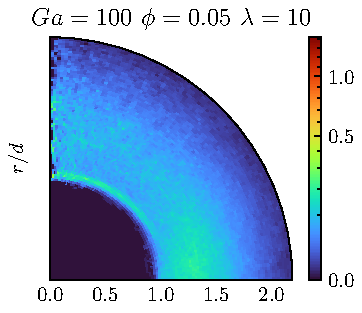
\includegraphics[height=0.21\textwidth]{image/HOMOGENEOUS_NEW/Dist/Pnst_l_10_Ga_100_PHI_0_05.pdf}
    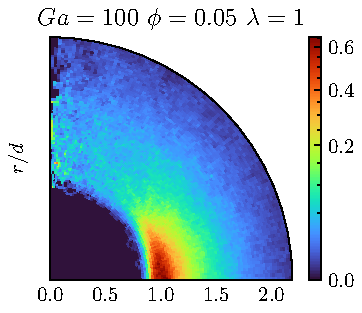
\includegraphics[height=0.21\textwidth]{image/HOMOGENEOUS_NEW/Dist/Pnst_l_1_Ga_100_PHI_0_05.pdf}
    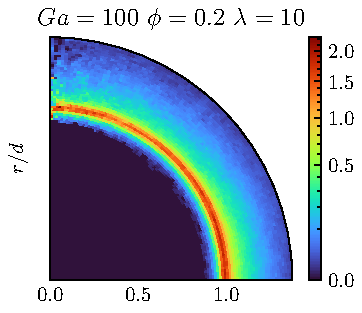
\includegraphics[height=0.21\textwidth]{image/HOMOGENEOUS_NEW/Dist/Pnst_l_10_Ga_100_PHI_0_2.pdf}
    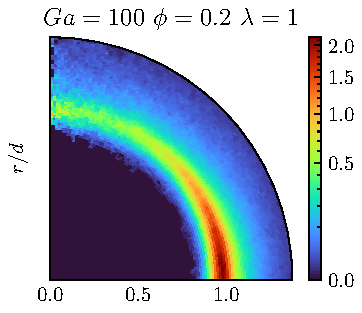
\includegraphics[height=0.21\textwidth]{image/HOMOGENEOUS_NEW/Dist/Pnst_l_1_Ga_100_PHI_0_2.pdf}
    \caption{Histogram of the normalized function $P_\text{nst}$ at high inertia $Ga = 100$.
    The color map represents the values of the nearest pair distribution function. %of $P_\text{nst}$.
    The origin corresponds to the position of the \textit{\textit{test particle}}.
    The dimensionless radial and azimuthal coordinates, $|\textbf{r}|/d$ and $\theta$, correspond to the nearest neighbor position.
    The vertical direction corresponds to the flow direction, which is also the axis of symmetry for $P_\text{nst}$.
    (left) Low volume fraction cases $\phi=0.05$ for $\lambda = 1,10$.
    (right) High volume fraction cases $\phi=0.2$ for $\lambda = 1,10$.}
    \label{fig:Pnst_high_Ga}
\end{figure}
%If we compare \ref{fig:Pnst_high_Ga} (right) with their counterparts from \ref{fig:Pnst_low_Ga} (right) we observe that $P^n_\text{r}$ becomes even larger at contact of the particles for $Ga=100$.
%Again, this could witness of the presence of clustering of particles. 
%In general, all $P_\text{nst}$ from \ref{fig:Pnst_high_Ga} exhibit some differences compared to the cases \ref{fig:Pnst_low_Ga}. 
%In the high inertial cases (\ref{fig:Pnst_high_Ga}), we can notice that $P_\text{nst}$ is larger on the sides of the \textit{test particle} for the iso-viscous emulsions ($\lambda = 1$).
Anisotropy in \ref{fig:Pnst_high_Ga} for $\lambda=1$ is particularly striking compared to \ref{fig:Pnst_low_Ga}. 
In the former, a higher concentration of particles is identified at $\theta \approx 0$, as seen in \ref{fig:Pnst_high_Ga}. 
A higher concentration of $P_\text{nst}$ around $\theta \approx 0$ indicates the presence of horizontal rafts of particles. 
In this case, the microstructure is non-homogeneous and anisotropic; this situation is illustrated in \ref{fig:scheme_clusters} (\textit{Case 3: ``layers''}). 
As the \textit{Galileo} number ($Ga$) increases and for low values of the viscosity ratio ($\lambda$), the probability of having neighbors on the horizontal plane of the \textit{test particle} increases. 
This leads to an increase in the anisotropy of the microstructure, which is more pronounced for low volume fractions. 
In contrast, the high-viscosity drops display an isotropic distribution of the nearest particles around the \textit{test particle}. 
This observation suggests the presence of isotropic clustering of particles.


%In comparison the high viscosity drops show an isotropic discitrbution of nearest particle around the \textit{test particle}. This could witness of the presence of isotropic clustering of particles.

%We do not observe a significant effect of the volume fraction on the anisotropy of the distribution.
%However, at this stage it remains unclear if increasing $\phi$ have a positive or negative impact on the anisotropy of the distribution. 

To illustrate the impact of $\lambda$ on the microstructure, \ref{fig:images} displays snapshots of two DNS at $\phi = 0.05$ and $Ga = 100$. 
As predicted by $P_\text{nst}$, we observe layers and particles in close contact for $\lambda = 1$, contrasting with the seemingly more evenly dispersed microstructure for $\lambda = 10$.
\begin{figure}[h!]
   \centering
   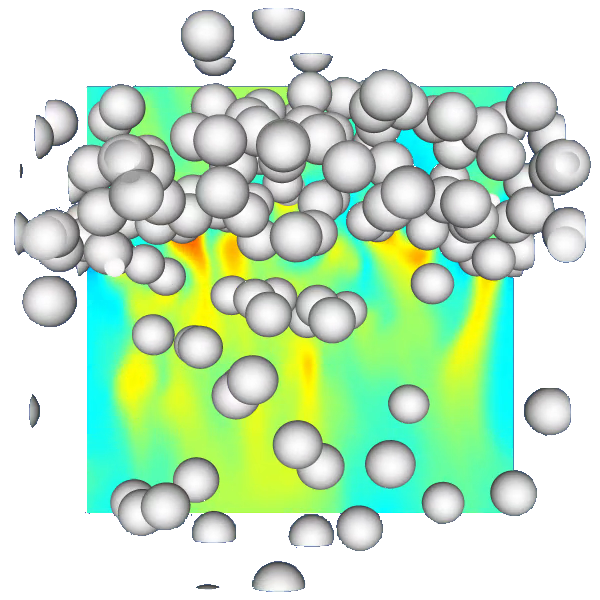
\includegraphics[width=0.4\textwidth]{image/HOMOGENEOUS_NEW/P_PHI_5_l_10_Ga_100.png}
   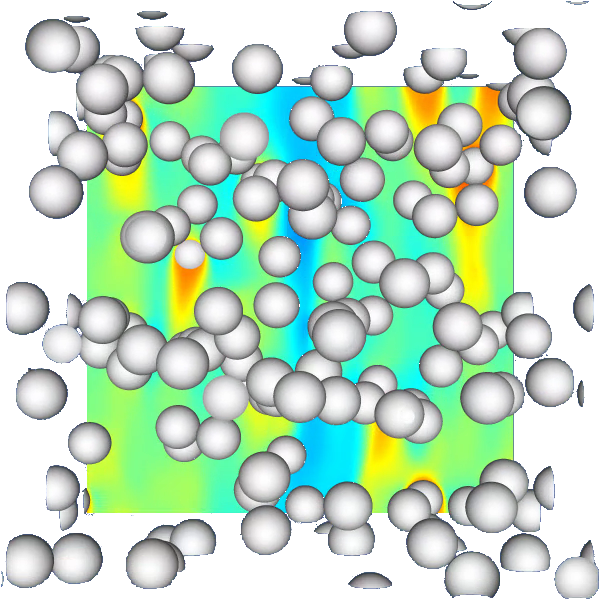
\includegraphics[width=0.4\textwidth]{image/HOMOGENEOUS_NEW/P_PHI_5_l_1_Ga_100.png}
   \caption{Snapshot of a simulation at $t^* = 150$ for $\phi=0.05$ and $Ga=100$.
   Color map : values of the vertical component of the velocity, field on the vertical plane defined by the equation $z=0$. 
   (left)  $\lambda = 1$.
   (right)  $\lambda = 10$.
   }
   \label{fig:images}
\end{figure}
In fact, for $\lambda = 10$, in \ref{fig:images} (right), we can still observe horizontal rafts of droplets or droplets rising side-by-side, but this effect is not as pronounced as for $\lambda = 1$. 
Drops with high viscosity ratios maintain a significant distance between other drops, which prevents the creation of structures such as droplet layers.
% This might be because of a higher vorticity around the viscous droplets.   
% As discussed in \citet{zhang2021three}, rising pairs of spherical bubbles may reach a stable side-by-side configuration, which tends to generate horizontal clusters.
% They range of dimensionless parameters is consistent with the ones presented in this study, making this hypothesis valuable for iso-viscous emulsions. 
% In \citet{legendre2003hydrodynamic} they study the interaction of a bubble pair rising side-by-side. 
% They stipulate that for two bubbles at moderate \textit{Reynolds} number $50-100$, the interaction forces are found to be repulsive, while it is attractive or null for higher \textit{Reynolds} number. 
% In our case it is reasonable to think that such pair attraction / repulsion mechanisms might drive the clustering mechanism.
%On another note, we can observe on \ref{fig:images} (left) that the distance between the layers is roughly equal to the length of the numerical domain. 
%Indeed, only one layer of droplets is present in the domain. 
%Therefore, the current microstructure is constrained by the size of the numerical domain, it is probably not representative of the real microstructure that we would obtain in an infinite non-periodic domain. 
%Additionally, one might argue that the layers appear due to collective effects drove by the size of the box.
%Indeed, it is exactly what we observe for small number of bubbles ($N_b = 4$) rising in a periodic domain, see \citet{loisy2017}. 
%However, we might expect that horizontal layers such as the one observed in \ref{fig:images} (left) still remain for lager boxes since the number of droplets is consequent.
%In our case, the presence of horizontal raft might be the consequence of pairwise interactions mechanism, as discussed above. 
%Therefore, it is likely that that layers still appear regardless of the size of the box.
%Nevertheless, the distance between these layers is still constrained by the size of the numerical domain, despite the consequent number of droplets used here. 
%In all rigor, DNS in a larger domain with more particles would be required to evaluate the microstructure dependence on the domain size. 
%Nevertheless, due to evident numerical constrains it has not been performed in this study.  
From the present analysis of $P_\text{nst}$ and the actual microstructure presented in \ref{fig:images} we can infer that the \textit{nearest particle statistics} is able to predict features in the microstructure such as layers and clusters. 


\subsection{Nearest particle radial distribution function }

Although \ref{fig:Pnst_low_Ga} and \ref{fig:Pnst_high_Ga} give a good qualitative representation of the particle-pair azimuthal distribution, they fall short in delivering a quantitative depiction of the radial distribution.
Thus, in this section we investigate the value of the radial distribution function $P_\text{r-nst}$ defined in \ref{eq:P_r}. 
For a random isotropic distribution of hard spheres, it is possible to derive a theoretical prediction for $P_\text{nst}$ obtained in the vanishing volume fraction limit. 
Indeed, it is shown in \citet{zhang2021ensemble} that for a dilute random arrangement of particles $P_\text{nst}(r)$, reads as
\begin{equation}
    P_\text{nst}^{\phi \ll 1}(r) = n_p e^{- 8\phi\left[(r/d)^3-1\right]}.
    \label{eq:Pnst_dilute}
\end{equation}
It must be understood that this formula is accurate only at $\mathcal{O}(\phi)$; therefore, in most cases, it is not expected to be representative.
Additionally, \citet{torquato1990nearest} derived a radial distribution function for hard spheres at arbitrary volume fractions $\phi$. In our notation, this distribution can be written
\begin{equation}
    P_\text{nst}^\text{th}(r) = 
        n_p\left(e+\frac{f}{(r/d)} +\frac{g}{(r/d)^2}\right)
    e^{-\phi\left[8e\left((r/d)^3-1\right)+12 f\left((r/d)^2-1\right)+24g\left((r/d)-1\right)\right]}
    \label{eq:torquato}
\end{equation}
with, 
\begin{align*}
    && e= \frac{1+\phi}{(1-\phi)^3},
    && f= \frac{-\phi (3+\phi)}{2(1-\phi)^3},
    && g= \frac{\phi^2}{2(1-\phi)^3}.
\end{align*}
%In both cases 
It should be noted that both \ref{eq:Pnst_dilute} and \ref{eq:torquato} are derived for hard spheres. 
%and may differs %from the droplet pair distribution.
In particular, for hard sphere $P_\text{nst}^\text{th} = 0$ for $r<d$ while in our case, particles might deform at contact, meaning that $P_\text{nst}$ is finite for certain $r<d$. 
However, using these theoretical probability density functions for comparative purposes remains valuable. 

\begin{figure}[h!]
    \centering
    % 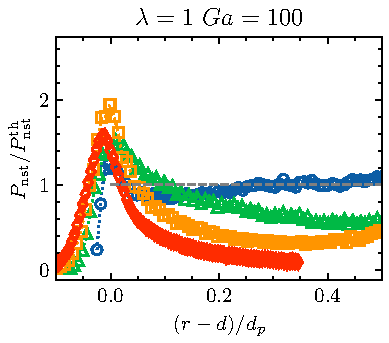
\includegraphics[height=0.3\textwidth]{image/HOMOGENEOUS_NEW/Dist/Pr_l_1_Ga_100.pdf}
    % 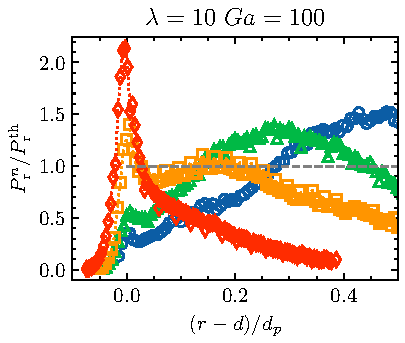
\includegraphics[height=0.3\textwidth]{image/HOMOGENEOUS_NEW/Dist/Pr_l_10_Ga_100.pdf}
    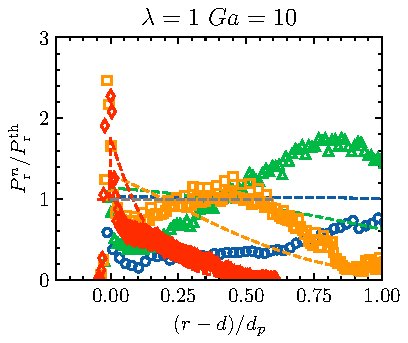
\includegraphics[height=0.3\textwidth]{image/HOMOGENEOUS_NEW/Dist/Pr_l_1_Ga_10.pdf}
    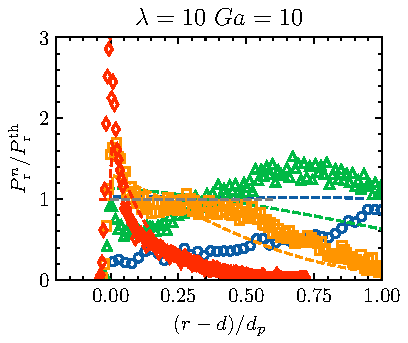
\includegraphics[height=0.3\textwidth]{image/HOMOGENEOUS_NEW/Dist/Pr_l_10_Ga_10.pdf}
    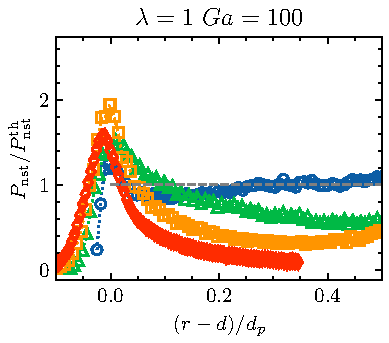
\includegraphics[height=0.3\textwidth]{image/HOMOGENEOUS_NEW/Dist/Pr_l_1_Ga_100.pdf}
    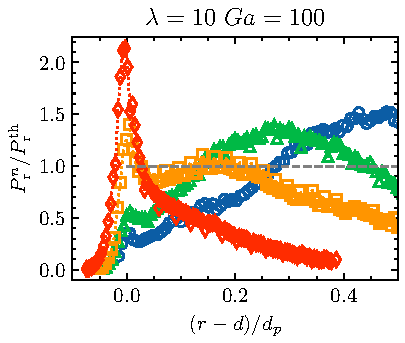
\includegraphics[height=0.3\textwidth]{image/HOMOGENEOUS_NEW/Dist/Pr_l_10_Ga_100.pdf}
    \caption{Radial probability density function divided by the theoretical distribution $P_\text{nst}^{\phi \ll 1}$ (\ref{eq:Pnst_dilute}), as functions of the dimensionless distance $r/d$, for $Ga = 100$, $Ga =10$, $\lambda = 1$ and $\lambda = 10$.
    (dashed lines) Theoretical prediction : $P_\text{nst}^{th}/P_\text{nst}^{\phi \ll 1}$. 
    (symbols) DNS results of $P_\text{r-nst}(r) / P_\text{nst}^{\phi \ll 1}$ with :
    ($\pmb\bigcirc$) $\phi = 0.01$; ($\pmb\triangle$) $ \phi = 0.05$; ($\pmb\square$) $\phi = 0.1$ ($\pmb\lozenge$) $\phi = 0.2$.
    For $r<d$ we arbitrarily set $P_\text{nst}^{\phi \ll 1} = 1$ so that $P_\text{r-nst}$ can be visualized. 
    }
    \label{fig:Pr}
\end{figure}
In \ref{fig:Pr}  we plot the radial distribution $P_\text{r-nst}$ as functions of the dimensionless distance $r/d$. 
We display two different viscosity ratios and multiple volume fractions. 
Let us first examine the low inertia cases displayed in \ref{fig:Pr} (top). 
It is seen that at $\phi = 0.01$ we have $P_\text{r-nst} < P_\text{nst}^{\phi\ll 1}$ for roughly $r/d < 2$.
This indicates that the likelihood of finding the nearest neighbor in the vicinity of the \textit{test particle} (i.e. $r/d<2$) is less than the random and dilute distribution.
In opposition, at $r/d>2$ the probability density $P_\text{r-nst}$ is higher than $P_\text{nst}^{\phi\ll 1}$ \eqref{eq:Pnst_dilute}.
In these cases ($\phi = 0.01$ and $\lambda = 10, 1$), the maximum of $P_\text{r-nst}$ is reached at $r/d \approx 3$, indicating that particles maintain on average a significant distance between each other. 
For comparison, the distance to the nearest neighbor in an ordered array of particles in a cubic lattice is  $\frac{1}{2}\left[4\pi/(\phi 3)\right]^{1/3} \approx 3.74$ at $\phi = 0.01$.
As $\phi$ increases, the maximum of $P_\text{r-nst}$ is found at lower values of $r/d$. 
At $\phi = 0.2$ the maximum of $P_\text{r-nst}$ is located at $r/d = 1$ which signifies that droplets are concentrated at the contact of the \textit{test particle}. 
At this stage, no differences between the cases $\lambda = 1$ and $\lambda = 10$ have been identified.

Let us now turn our attention to the inertial cases displayed on \ref{fig:Pr} (bottom). 
In the dilute regime ($\phi = 0.01$) and for $\lambda=1$, we observe that $P_\text{r-nst}$ is in complete agreement with the random and dilute distribution $P_\text{nst}^{\phi \ll 1}$ \eqref{eq:Pnst_dilute}.  
In contrast, when $\lambda = 10$ at the same $\phi$ and $Ga$, it becomes evident that fewer particles gather in close vicinity to the \textit{test particle}. 
% Consequently, on average, the droplets are positioned at greater distances from each other compared to the dilute random distribution. 
For $\lambda = 10$ a behavior analogous to the low inertia scenario is observed. 
Indeed, the peak of $P_\text{r-nst}$ shifts leftward with increasing values of $\phi$, until the maximum of $P_\text{r-nst}$ is found at $r/d = 1$ for $\phi = 0.2$.
For $\lambda = 1$, we observe that $P_\text{r-nst}$ becomes progressively lower than the dilute and random distribution for increasing values of $\phi$ and moderate values of $r/d$. 
However, the maximum of $P_\text{r-nst}$ in these cases is located at $r/d = 1$ regardless of $\phi$. 
Thus, in the inertial and low viscous regime, the nearest neighbor is more likely to be located at near contact with the \textit{test particle}. 
Additionally, it is clear from \ref{fig:Pr} that the particles deform at contact, as witnessed by the non-vanishing value of $P_\text{r-nst}$ for $r/d<1$.
This phenomenon is particularly pronounced for the case $Ga = 100$ and $\lambda =1$. 
This is consistent with the high values of droplet aspect ratios reported in \ref{ap:deformation} \ref{fig:chi} for this case.
Interestingly, we note that in this case $P_\text{r-nst}$ exhibits the same values in the region $r/d <1$ for all values of $\phi$. 



To conclude these observations, we note that both the radial and azimuthal distributions were affected by the inertial effects measured by the \textit{Galileo} number. 
The major effect of high inertia is the generation of strong anisotropy in the particle pair distribution and a more important concentration of neighboring particles at $r/d < 1$. 
Furthermore, the density at contact of the \textit{test particle} is higher for increasing volume fractions. 
The viscosity ratio strongly impacts the microstructure, but only at high $Ga$, whereas at low $Ga$, the change in viscosity ratio has no notable impact on $P_\text{nst}$. 
Lastly, note that \ref{eq:torquato} provides a significantly improved prediction of the radial distribution compared to $P_\text{nst}^{\phi \ll 1}$ \eqref{eq:Pnst_dilute} (see \ref{fig:Pr}). 
Indeed, the DNS results show that $P_\text{r-nst}$ follows trends similar to $P_\text{nst}^\text{th}$ as $\phi$ increases. 
Quantitative agreements are particularly observed for high inertia cases.

\subsection{Macroscopic modeling of the microstructure}
%Up to now we have presented visualizations of the microstructure with 2D or 1D distributions. 
%For a more concise description we would like to adopt a different approach. 
%Following \citet{zhang2023evolution} we opt to describe the microstructure using the second moment of $P_\text{nst}$ with respect to \textbf{r}, which reads
Until now, we have depicted the microstructure through 2D or 1D distributions. To provide a more succinct description, we propose a different method. 
Inspired by \citet{zhang2023evolution}, we will characterize the microstructure using the second moment of $P_\text{nst}$ with respect to $\mathbf{r}$, which is expressed as
\begin{equation}
    \textbf{R} =\frac{1}{n_p} 
    % \int_0^\infty 
    \int_{\mathbb{R}^3} 
    \textbf{rr} P_\text{nst}(\textbf{r}) d\textbf{r}.
    \label{eq:R}
\end{equation}
The tensor $\textbf{R}$ allows us to measure the mean-square distance between a particle and its nearest neighbor in the three dimensions of space.
%This second-rank tensor measures the spread of the nearest neighbor distribution in a given direction. 
It is worth noting that such a quantity is computable only because $\lim_{|\textbf{r}|\to \infty} P_\text{nst}(\textbf{r}) = 0$, which enables the integral of \ref{eq:R} to converge. 
This would not be the case for classical pair distributions, which is one of the main reasons for using the \textit{nearest particle statistics} framework. Since our objective is to measure the anisotropy of the microstructure, we are particularly interested in the deviatoric part of this tensor, namely
\begin{equation*}
    \textbf{A} = \textbf{R} - \frac{1}{3}  \text{tr}(\textbf{R}) \bm\delta.
\end{equation*}
Where $\bm\delta$ is the unit tensor and 
$\textbf{A}$ represents the likelihood of having a particle in a given direction compared to the mean radial square distance. 
Therefore, in an isotropic suspension, we have $A_{xx} = A_{yy} = 0$, where $y$ represents the coordinate aligned with gravity. 
In a situation like the one depicted in \ref{fig:images} (left), particles are more likely to have closer neighbors on the lateral sides rather than vertically positioned, hence  $A_{yy} < 0$ and $0 < A_{xx}$. 


To facilitate the understanding of the subsequent findings, it is helpful to calculate the distance $r_m$. 
This distance represents the average distance to the closest neighboring particle within a random arrangement of dilute hard spheres. 
Through direct integration of \ref{eq:Pnst_dilute}, we get
\begin{align}
    \frac{r_m^2}{d^2}
    = 
    % \frac{1}{n_p}
    \frac{1}{d^2}
    \int_{\mathbb{R}^3} r^2 P_\text{nst}^{\phi \ll 1}(\textbf{r}) d\textbf{r} 
    =  \frac{\Gamma\left({{5}\over{3}} , 8\,\phi\right)}{8^{2/3}}\frac{e^{8\phi}}{\phi^{2/3}},
    % = d^2{{4^{{{2}\over{3}}}\,\Gamma\left({{5}\over{3}} , 8\,\phi\right)
    % \,e^{8\,\phi}}\over{2^{{{10}\over{3}}}\,\phi^{{{2}\over{3}}}}}
\end{align}
where $\Gamma(z,a) = \int_a^\infty t^{z-1} e^{-t} dt$ is the upper incomplete gamma function.
\begin{figure}
  \centering
  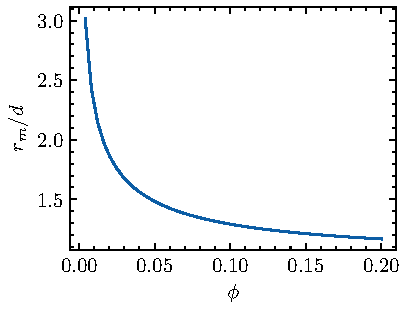
\includegraphics[height = 0.3\textwidth]{image/HOMOGENEOUS_NEW/PA/rm.pdf}
  \caption{Dimensionless radial distance to the nearest neighbor for a random distribution.}
  \label{fig:agee}
\end{figure}
Since the upper incomplete gamma function is relatively uncommon, we have illustrated the dimensionless distance $r_m/d$ as a function of $\phi$ in \ref{fig:agee} to aid understanding. This figure clearly shows that $r_m$ decreases as $\phi$ increases.
%Since the upper incomplete gamma function is not so common we have plotted in \ref{fig:ap:agee} the dimensionless distance $r_m/d$ in terms of $\phi$ to help comprehension. As can be seen from this figure $r_m$ is a decreasing function of $\phi$.

\begin{figure}[h!]
    \centering
    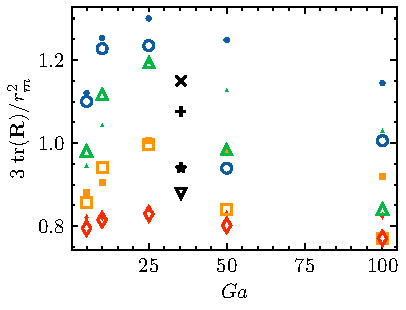
\includegraphics[height=0.3\textwidth]{image/HOMOGENEOUS_NEW/PA/trR.pdf}
    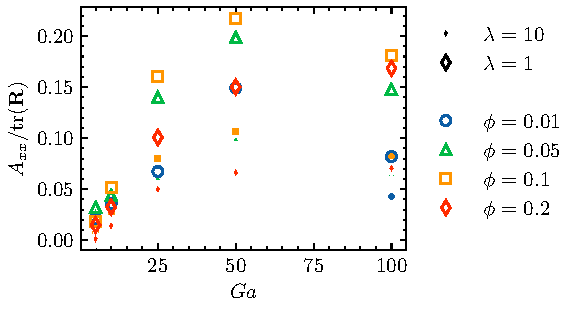
\includegraphics[height=0.3\textwidth]{image/HOMOGENEOUS_NEW/PA/Axx.pdf}
    \caption{
        (left) Dimensionless trace of $\textbf{R}$ as a function of the volume fraction.%Trace of the second moment of the probability density function $P_\text{nst}(\textbf{r})$ divided by the square diameter of the particles $d^2$. 
        (right) Horizontal components of the anisotropy tensor divided by the trace of $\textbf{R}$. %the second moment of the probability density function.
    ($\pmb\bigcirc$) $\phi = 0.01$; ($\pmb\triangle$) $ \phi = 0.05$; ($\pmb\square$) $\phi = 0.1$ ($\pmb\lozenge$) $\phi = 0.2$.
    The hollow symbols correspond to $\lambda = 1$, the filled symbols to $\lambda = 10$.
    % For $r<d$, we arbitrarily set $P_\text{nst}^\text{th} = 1$ so that the distribution can be visualized.
    Black symbols represent the results of \citet{zhang2023evolution} for sedimenting spherical particles with $\phi = 0.016,0.056,0.134,0.262$ and $\zeta = 2.56$. %$\phi = 0.0168,0.0565,0.1341,0.2622$ 
    Corresponding to $\pmb\times,\pmb +, \pmb\star , \pmb\triangledown$, respectively.
    }
    \label{fig:A}
\end{figure}
In \ref{fig:A} (left), the dimensionless mean square distance between nearest neighbors, represented as $3\cdot\text{tr}(\textbf{R})/r_m^2 = \textbf{R}:\bm\delta/r_m^2$, is illustrated for all configurations explored in this study. 
The simulation marked by the symbol \textcolor{col1}{$\pmb\circ$} in \ref{fig:A} (left), corresponding to parameters $\lambda = 1$, $Ga = 100$, and $\phi = 0.01$, yields a value of $\bm\delta:\textbf{R}/r_m^2 \approx 1$. 
This observation agrees with the quasi-hard-sphere distribution previously reported in this case in \ref{fig:Pr} (left).
The dependence of the mean square distance on the volume fraction is also displayed on \ref{fig:A} (left). 
We observe a decrease in $\bm\delta:\textbf{R}/r_m^2$ as $\phi$ increases, indicating that particles tend to come closer to each other on average compared to a dilute random distribution of hard spheres. 
This observation, as highlighted by \citet{zhang2023evolution}, suggests the emergence of clusters when increasing the particle volume fraction. 
The dependence on the \textit{Galileo} number is non-monotonic. 
Indeed $\bm\delta:\textbf{R}/r_m^2$ increases until $Ga = 25$ and then decreases until $Ga = 100$. We also note that the distance to the nearest neighbor is not significantly affected by the viscosity ratio, particularly when dealing with high-volume fractions. 
In \ref{fig:A} (left), the symbols $\pmb\star$, $\pmb\times$, $\pmb +$, and $\pmb\triangledown$ depict the findings from the study conducted by \citet{zhang2023evolution} on the sedimentation of solid spheres in a liquid.
As observed, the value of $\textbf{R}:\bm\delta$ is, on average, closer to the mean $r_m^2$ than our simulations, but it maintains the same trend, i.e., clusters appear as the volume fraction increases.
 
\ref{fig:A} (right) illustrates the anisotropy of the microstructure. We can see on \ref{fig:A} (right) that we have $A_{xx} \ge 0$ for nearly all our cases, meaning that the emulsion is either isotropic ($A_{xx} = 0$), or exhibits a tendency towards a horizontal alignment of particles on average ($A_{xx} >0$). % or with particles that are in average more aligned horizontally ($A_{xx} >0$). 
%Moreover $A_{xx}$ increases with $Ga$ until $Ga = 50$ where we reach a maximum, and then decrease until $Ga =100$  but still remains consequent. 
Additionally, $A_{xx}$ rises with $Ga$ up to $Ga = 50$, reaching a peak, and subsequently decreases until $Ga = 100$, although it remains significant.
In agreement with the remarks of the previous section, the value of $A_{xx}$ is greater for $\lambda = 1$ and lower for  $\lambda = 10$.
Although not obvious at first, we observe a non-monotonic trend with the volume fraction. $A_{xx}$ increases up to a peak value at $\phi = 0.1$ (indicated by \textcolor{col3}{$\pmb\square$} on \ref{fig:A} (right)), but then decreases for $\phi=0.2$ (shown by the \textcolor{col4}{$\pmb\lozenge$} symbols). %$A_{xx}$ first increases up to a maximum value for $\phi =0.1$ (represented by \textcolor{col3}{$\pmb\square$} on \ref{fig:A} (right)) and then decreases for $\phi=0.2$ (represented by the \textcolor{col4}{$\pmb\lozenge$} symbols).
%Although, it is not quite obvious we observe a non-monotonic trend with the volume fraction, $A_{xx}$ first increases up to a maximum value for $\phi =0.1$ (represented by \textcolor{col3}{$\pmb\square$} on \ref{fig:A} (right)) and then decreases for $\phi=0.2$ (represented by the \textcolor{col4}{$\pmb\lozenge$} symbols). 
This implies that at a certain volume fraction, around $\phi \approx 0.1$, higher $\phi$ makes the microstructure more isotropic, while at low volume fraction ($\phi < 0.1$), increasing $\phi$ favors the side-by-side configuration.
This phenomenon of isotropization at high $\phi$ has been reported in other studies such as in \citet{seyed2021sedimentation} for sedimentation of solid particles. 
However, at high \textit{Galileo} numbers, it seems that this effect is less pronounced. 


To conclude, we classify the microstructure into four classes :
(1) The homogeneous microstructure.
(2) The non-homogeneous but isotropic microstructure with $\textbf{R}:\bm\delta > r_m^2$, or dispersed arrangement. %ordered array.
(2 bis) The non-homogeneous but isotropic microstructure with $\textbf{R}:\bm\delta < r_m^2$, or clustering. 
(3) The non-homogeneous and non-isotropic microstructure or layering ($\textbf{A}\neq \textbf{0}$). 
Each of these types is characterized by specific values of $\textbf{R}$; they are reported in \ref{tab:microstructure}. 

\begin{table}[h!]
    \caption{Microstructure classification}
    \label{tab:microstructure}
    \centering
    \begin{tabular}{|lccccc|} \hline
        Microstructure types & Homogeneous & Isotropic & \ref{fig:scheme_clusters} & $\textbf{R}:\bm\delta/r_m^2$ & $A_{xx}/tr(\textbf{R})$ \\
        Homogeneous & Yes & Yes &(\textit{Case 1}) & $ \approx 1$ & $\approx 0$ \\
        Dispersed &  No & Yes  &(\textit{Case 2}) & $ > 1$ & $\approx 0$ \\
        Clustering &  No & Yes  &(\textit{Case 2}) & $ < 1$ & $\approx 0$ \\
        Layering &    No & No  &(\textit{Case 4}) & $ - $ & $< 1$\\ \hline
    \end{tabular}
\end{table}
Additionally, to highlight the dependence of $\textbf{R}$ on $\phi$ and $Ga$, we display the values of $A_{xx}/tr(\textbf{R})$ and $\textbf{R}:\bm\delta/r_m^2$ in phase diagrams on \ref{fig:phase}.
We observe that the mean square particle distance compared to a random case decreases when increasing the volume fraction and is globally higher for viscous particles ($\lambda = 10$).
Meanwhile, the likelihood of finding the nearest neighboring particle on the horizontal is greater for $\lambda=1$ than $\lambda = 10$, and it is globally increasing with  $Ga$ and non-monotonic with $\phi$. 
We reach the configuration with the maximum anisotropy for both viscosity ratios at $Ga \approx 50$ and $\phi \approx 0.1$. 
%We conclude that 

\begin{figure}[h!]
    \centering
    \begin{tikzpicture}[scale=0.8]
        \node (img) at (0,0) {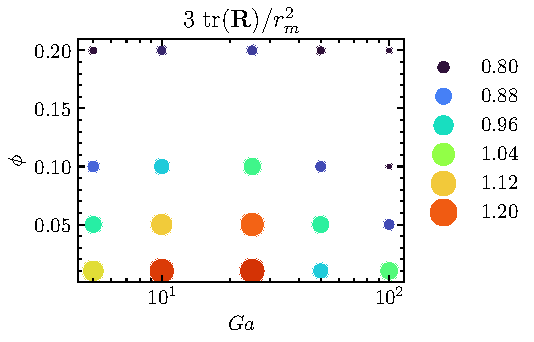
\includegraphics[height=5.5cm]{image/HOMOGENEOUS_NEW/PA/phase_Rtr_l_1.pdf}};
        % \draw[dashed] (10cm,-1.6) ellipse (3 and 2);
        \node (txt) at (-2,1) {Clustering};
        \node (txt) at (-1,-1.6) {Dispersed};
        \draw[dashed] ($(-1,-1.6) + (-10:3 and 2)$(P) arc
        (-10:155:3 and 2);
        \node (img) at (10.5,0) {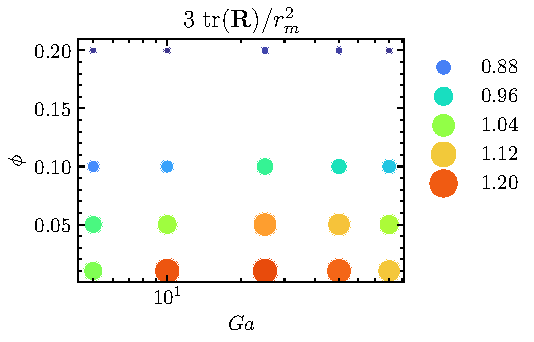
\includegraphics[height=5.5cm]{image/HOMOGENEOUS_NEW/PA/phase_Rtr_l_10.pdf}};
        % \draw[dashed] (10cm,-1.6) ellipse (3 and 2);
        \node (txt) at (8.5,1) {Clustering};
        \node (txt) at (10,-1.6) {Dispersed};
        \draw[dashed] ($(10,-2) + (-10:3 and 2)$(P) arc
        (-10:180:3 and 2);
    \end{tikzpicture}
    \begin{tikzpicture}[scale=0.8]
        \node (img) at (0,0) {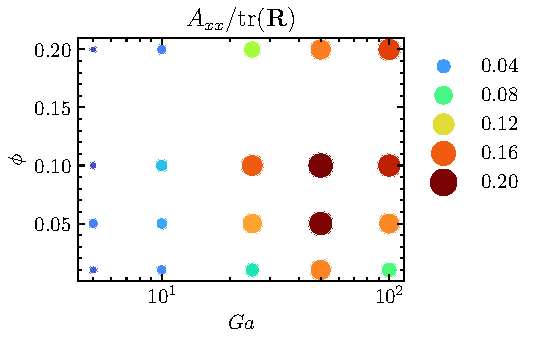
\includegraphics[height=5.5cm]{image/HOMOGENEOUS_NEW/PA/phase_axx_l_1.pdf}};
        \draw[dashed] (1.2,0.3) ellipse (1.5 and 2.5);
        \node (txt) at (1.2,1) {Anisotropic};
        \node (txt) at (-2,1) {Isotropic};

        \node (img) at (10.5,0) {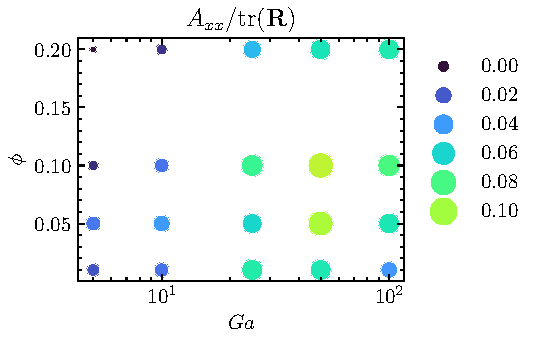
\includegraphics[height=5.5cm]{image/HOMOGENEOUS_NEW/PA/phase_axx_l_10.pdf}};
        % \draw[dashed] (11.7,-0.5) ellipse (0.75 and 1.75);
        % \node (txt) at (11.7,1) {Anisotropic};
        \node (txt) at (8,1) {Isotropic};
    \end{tikzpicture}
    \caption{
        (top) Phase diagram of the dimensionless mean square distance to the nearest neighbor, $\bm\delta:\textbf{R}/r_m^2$.
        (bottom) Phase diagram of the dimensionless horizontal components of the anisotropy tensor, $A_{xx}/\text{tr}(\textbf{R})$.  
        (left) Iso-viscous emulsion $\lambda = 1$.
        (right) Viscous droplets $\lambda = 10$ }
    \label{fig:phase}
\end{figure}

\subsubsection*{Discussion}
%Although, previous studies mainly focused on bubbles or solid particles, it is reasonable to compare the $\lambda = 1$ and $\lambda = 10$ simulations, to the former and the latter cases, respectively. 
%In \citet{bunner2002dynamics} they performed tri-periodic simulation of buoyant bubbles at $Re \approx 10-30$ for various $\phi$.
%They reported a preference for the bubbles to be aligned in pair.
While earlier studies primarily focused on bubbles or solid particles, it is reasonable to draw parallels between simulations with $\lambda = 1$ and $\lambda = 10$, corresponding to the former and latter scenarios, respectively. In \citet{bunner2002dynamics}, buoyant bubbles were simulated in a tri-periodic setup at Reynolds numbers around 10-30 for various volume fractions ($\phi$). The authors noted a tendency for the bubbles to align in horizontal pairs. % a finding that aligns with our observations.
This observation is consistent with what we observe in \ref{fig:phase} ($\lambda = 1$) since the anisotropy tensor is relatively high ($A_{xx} \approx 0.15$) for $Ga = 25$ (which corresponds roughly to $Re = 25$). 
% Additionally, it is seen that these layers structures are lost at lower volume fraction ($\phi = 0.01$). 
Moreover, \citet{zhang2021direct} conducted Direct Numerical Simulations (DNS) of buoyant bubbly flows within tri-periodic domains. The Reynolds numbers varied from $Re=18$ to $22.8$ across different volume fractions, $\phi$, ranging from $0.05$ to $0.2$, with a fixed Galileo number, $Ga$, of $29$. They observed the presence of anisotropic clusters for $\phi > 0.1$, while noting their absence at lower volume fractions. This observation aligns with findings depicted in \ref{fig:phase} (left), where a small decrease in the value of $A_{xx}$ may be observed for the lowest $\phi$.
%Furthermore, in \citet{zhang2021direct} they carried out DNS of buoyant bubbly flows in tri-periodic domains.
%Their \textit{Reynolds} numbers range form $Re=22.5\to 18$ for various volume fraction : $\phi = 0.05\to 0.2$ and a fixed \textit{Galileo} number of $Ga = 29$. 
%They observe anisotropic clusters for $\phi >0.1$ as well, and they report that at lower volume fraction these structures are not present. 
%It is consistent with the results reported in \ref{fig:phase} (left) where we can see that the value of $A_{xx}$ clearly decreases for lower $\phi$. 

For solid particles at $Ga = 144$, it is observed in \citet{shajahan2023inertial} that vertical rafts of particles are formed in the dilute regime ($\phi \approx 0.02$). This phenomenon was attributed to a well-defined wake around individual particles, which effectively traps neighboring particles within the wake without causing repulsion toward the sides. %This effect was explained by the presence of a more developed wake for dilute solid particles which trap neighboring particles within the wake without repulsing it on the sides. 
In our case, we notice a greater concentration of particles in the vertical directions for $\lambda = 10$ compared to $\lambda = 1$ at $Ga = 100$, as evidenced by the smaller value of $A_{xx}$ in the former case. Although not immediately apparent, this phenomenon could be attributed to similar factors, namely, the wake of the viscous drop potentially inducing fewer instances of particles aligning side-by-side and more instances of vertically stable configurations. DNS at higher $Ga$ and $\lambda$ would be necessary to confirm or not the presence of the wake trapping effect. %To conclusively confirm or refute the presence of this wake-trapping effect, it would be necessary to conduct DNS at higher $Ga$ and $\lambda$ values.
%In our case we observe more particles in the verticals directions for $\lambda = 10$ than $\lambda =1$ at $Ga =100$, since $A_{xx}$ is smaller in the former cases.
%Although it is not quite obvious it might be the consequence of the same effects, i.e., the wake of the viscous drop might induce less side-by-side configuration and more vertical nearly stable configuration. 
%DNS at higher $Ga$ and $\lambda$ would be necessary to confirm or not the presence of the wake trapping effect.
%In our case we could not observe such a phenomenon, meaning that it might arise at larger \textit{Galileo} number or that the approximation of solid particle at for $\lambda = 10$ is too coarse.
In the moderately dense regime,  $0.02 < \phi \le 0.1$  \citet{shajahan2023inertial} identified more configurations of particles situated side-by-side. 
As mentioned above, even if it is less pronounced than for $\lambda = 1$, we indeed observe that $A_{xx}$ is higher in these cases; see \ref{fig:phase} (right). 
Additionally, \citet{almeras2021statistics} carried out experiments of liquid-solid fluidized bed with spherical particles. 
Their Reynolds numbers range between $150\leq Re \leq 360$ depending on the volume fraction $0.14 \leq \phi \leq 0.42$.
It is observed that particles are most concentrated on the horizontal plane of the reference particle when $\phi = 0.14$.
If the $\lambda = 10$ cases follow the same trend, it is reasonable to expect that the probability of horizontal configurations, already predominant at $Ga =100$, will continue to increase for higher \textit{Galileo} at $\phi  \approx 0.1$.

We would like to end this comparison with the literature with the study of \citet{yin2008lattice} which compares the microstructure of suspensions of rising bubbles with suspensions of sedimenting solid particles.
%They studied two \textit{Reynolds} numbers and two volume fractions : $Re = 5,20$ and  $\phi = 0.05, 0.2$, respectively.
%It is found that :
The study encompasses two Reynolds numbers ($Re = 5, 20$) and two volume fractions ($\phi = 0.05, 0.2$). Their findings reveal that: 
\enquote{    
     microstructure in bubble
    suspensions is more anisotropic and inhomogeneous than
    solid particle suspensions of the same volume fraction and
    \textit{Reynolds} number.    
}. 
%Although we compare emulsions with varying droplets' viscosity rather than bubbles and solid particles' suspension, our conclusion regarding the anisotropy of the flow is consistent with their study.
%Additionally, it is also observed in \citet{yin2008lattice} that the microstructure shape has a clear impact on the mean rising velocity of the dispersed phase.
%Indeed, they observed that a power-law function of $(1-\phi)$ fit perfectly the rising velocity of random and isotropic suspensions, while it is not the case when the microstructure exhibit anisotropic structures. 
%Therefore, as stated in introduction, the knowledge of the microstructure shape (reported in \ref{fig:phase}), is of utmost importance in the objective of building realistic averaged models. 
While our analysis focuses on emulsions with varying droplet viscosities rather than bubbles and suspended solid particles, our findings regarding the flow anisotropy align with the study of \citet{yin2008lattice}. 



% In the following we try to explain the origin of the striking difference between $\lambda = 1$ and $\lambda = 10$ on the particle pair distribution.
% With this objective in mind, we present a meticulous analysis of the particle time of interaction as well as the particles relative averaged velocity fields. 
